\documentclass[conference,a4paper]{IEEEtran}
\pdfminorversion=6
\usepackage[T1]{fontenc}
\usepackage[utf8]{inputenc}
\usepackage{graphicx,booktabs,tabularx,amsmath,amssymb,tikz,url,cite}
\usetikzlibrary{arrows.meta}
\usepackage[hidelinks]{hyperref}
\newcolumntype{Y}{>{\raggedright\arraybackslash}X}
\begin{document}
\title{Parameter-Efficient Radiograph--History Classification with Class-Aware Alignment and Bidirectional Fusion}
\author{\IEEEauthorblockN{Nguyen Van Le Ba Thanh, Nguyen Gia Kiet, Ly Quoc Ngoc, Do Thi Thanh Ha}
\IEEEauthorblockA{Faculty of Information Technology, University of Science\\
Vietnam National University Ho Chi Minh City, Ho Chi Minh City, Vietnam}}
\maketitle

\begin{abstract}
Adapting medical vision--language models to small musculoskeletal datasets requires balancing contextual information, class imbalance, and optimization cost. Earlier image--text pretraining methods improve transferable representations, but do not establish whether a more complex downstream fusion recipe is justified. We study XBone-Net, which adapts BiomedCLIP through two offline phases: class-aware soft image--text matching with low-rank adapters, followed by bidirectional global-to-local cross-attention and linear classification. Online inference uses fixed weights on a radiograph and its clinical history. Across three seeds, XBone-Net reaches Macro-F1 of $0.5727\pm0.0193$ on the 22-class CTCH dataset and $0.6240\pm0.0118$ on the 10-class BTXRD dataset, while updating approximately 4.13\% of parameters. The CTCH test set contains 669 patients; BTXRD uses 750 test images and metadata-derived text. Recomputed, aligned predictions show higher observed Macro-F1 than the tested baselines, but paired tests do not establish superiority over fully tuned BiomedCLIP, Phase-2-only training, or concatenation. The results support parameter-efficient adaptation and identify unresolved component effects and generalization limits.
\end{abstract}
\begin{IEEEkeywords}
medical vision--language learning, radiograph classification, low-rank adaptation, cross-attention, class imbalance
\end{IEEEkeywords}

\section{Introduction}
Musculoskeletal classification can benefit from clinical context that is absent from pixels, such as the presenting complaint and prior history. Yet a small, imbalanced training cohort provides limited evidence for adapting a large biomedical model. Accuracy alone may favor common diagnoses, and a higher mean score need not justify a more complex architecture. The problem is therefore both methodological and empirical: how should a pretrained model combine a radiograph with history, and what benefit is supported by the available comparisons?

Research has progressed from supervised visual networks \cite{ResNet,DenseNet} to transferable image--text representations. CLIP established large-scale natural-language supervision \cite{CLIP}; ConVIRT brought paired contrastive learning to medicine \cite{ConVIRT}. GLoRIA introduced local image--word interactions, while MedCLIP addressed semantic false negatives \cite{GLoRIA,MedCLIP}. BiomedCLIP and BIOMEDICA then extended the scale and breadth of biomedical pretraining \cite{BiomedCLIP,BIOMEDICA}. These advances supply strong initial representations, but their benchmark results do not directly determine adaptation performance on a long-tailed radiograph--history classification task.

We study XBone-Net as a constrained downstream recipe. First, low-rank adaptation (LoRA) \cite{Hu2022LoRA} learns soft image--text correspondence using class-aware batches. Second, a global token in each modality queries local tokens of the other before linear classification. Effective-number weighting \cite{Cui2019ClassBalanced} and label smoothing define the supervised risk. The method uses native BiomedCLIP image tokens and a linear head; it requires no lesion annotation.

The contributions are \textbf{C1}, an explicit offline/online framework for parameter-efficient radiograph--history adaptation; \textbf{C2}, a training recipe that combines class-aware correspondence with conditional fusion; and \textbf{C3}, a matched empirical assessment against six external baselines and internal alternatives. The contribution is the task-specific integration and evaluation of established mechanisms. We do not claim a new foundation model, a new general attention mechanism, or universal superiority.

\section{Related Works}
The shift from image-only supervision to paired pretraining made reports useful even when downstream labels were scarce. ConVIRT achieved 89.0\% AUC on MURA with full-data fine-tuning \cite{ConVIRT}. GLoRIA moved beyond global alignment toward local image--word relations \cite{GLoRIA}. However, correspondence by patient identity can still treat clinically similar examples as negatives. MedCLIP's semantic matching addresses that issue and supports unpaired training \cite{MedCLIP}. XBone-Net adopts a simpler downstream construction based on the available class labels; this is a coarse semantic prior, not a replacement for medical knowledge extraction.

Broader pretraining further changes the available initialization. BiomedCLIP uses a large scientific image--caption corpus, and BIOMEDICA expands access and coverage \cite{BiomedCLIP,BIOMEDICA}. Captions still differ from the histories available at prediction time. Table~\ref{tab:related} summarizes this progression, with numerical results tied to their original evaluation settings. We evaluate the downstream adaptation recipe locally rather than comparing incompatible published numbers.

LoRA addresses the number of optimized weights; class-balanced loss addresses unequal class frequencies \cite{Hu2022LoRA,Cui2019ClassBalanced}. Neither implies that additional fusion improves classification. This motivates reporting parameter counts alongside internal comparisons and paired uncertainty estimates.

\begin{table*}[t]
\caption{Related work by principle, method, performance, and practical trade-off. Published protocols differ from ours. GLoRIA's numeric result is the re-evaluation in MedCLIP, Table 2; all other entries refer to the named work.}
\label{tab:related}
\centering\footnotesize
\begin{tabularx}{\textwidth}{@{}p{17mm}YYYYY@{}}
\toprule
Work & Principle & Method & Performance: data / measure / result & Pros & Cons \\
\midrule
ConVIRT \cite{ConVIRT} & Paired transfer & Global bidirectional contrastive loss & MURA; full-data fine-tuning; AUC 89.0\% & Label-efficient visual learning & Semantic negatives remain \\
GLoRIA \cite{GLoRIA,MedCLIP} & Local correspondence & Image-region / word alignment & RSNA; linear classification; accuracy 79.81\% & Retains local interactions & Paired-data requirement; no CTCH result \\
MedCLIP \cite{MedCLIP} & Semantic matching & Unpaired learning with medical knowledge & RSNA; linear classification; accuracy 80.75\% & Reduces false-negative supervision & Chest-domain evidence; semantic labels needed \\
BiomedCLIP \cite{BiomedCLIP} & Broad biomedical transfer & ViT/text encoders; PMC-15M pretraining & RSNA; 10\%-label linear probe exceeds fully supervised BioViL (reported) & Reusable biomedical initialization & Scientific captions differ from histories \\
BIOMEDICA \cite{BIOMEDICA} & Scale and open access & Literature curation; continued CLIP training & 40-task evaluation; average zero-shot gain 6.56\% (reported) & Broad, accessible resources & Not evaluated on CTCH in this study \\
\bottomrule
\end{tabularx}
\end{table*}

\section{Methods}
\subsection{Offline and Online Framework}
Let $\mathcal D=\{(x_i,t_i,y_i)\}_{i=1}^N$, where $x_i$ is a radiograph, $t_i$ is clinical history, and $y_i\in\{1,\ldots,K\}$. Offline training fits the encoders, fusion, and classifier, using validation data for checkpoint selection. Online inference applies fixed weights to a new pair (Fig.~\ref{fig:framework}). CTCH text uses prepared English translations of the reason for admission, disease history, and prior history; imaging findings, professional diagnosis, and labels are excluded. BTXRD text is generated from metadata and evaluated as a separate synthetic-text setting.

\begin{figure}[t]
\centering\resizebox{\columnwidth}{!}{
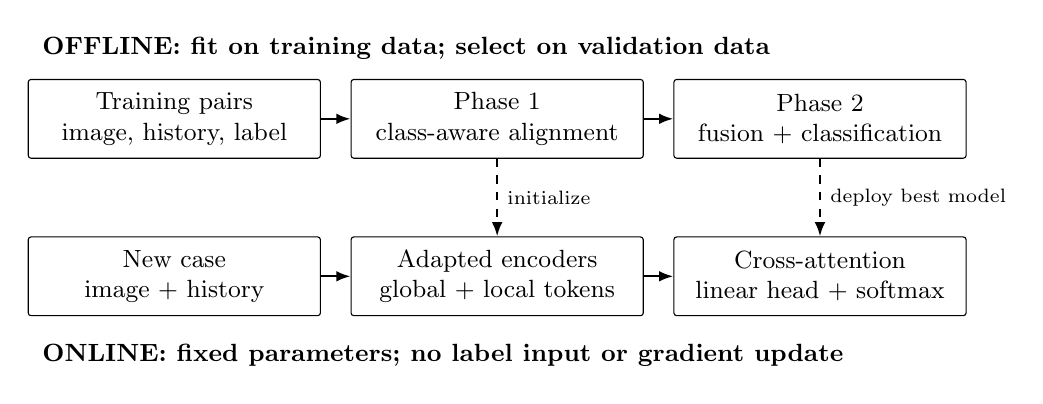
\begin{tikzpicture}[font=\small,
 box/.style={draw,rounded corners=1pt,align=center,minimum height=10mm,text width=35mm,inner sep=3pt},
 arr/.style={-{Latex[length=1.8mm]},thick}]
\node[box] (data) at (0,0) {Training pairs\\image, history, label};
\node[box] (p1) at (4.1,0) {Phase 1\\class-aware alignment};
\node[box] (p2) at (8.2,0) {Phase 2\\fusion + classification};
\draw[arr] (data)--(p1); \draw[arr] (p1)--(p2);
\node[box] (new) at (0,-2.0) {New case\\image + history};
\node[box] (enc) at (4.1,-2.0) {Adapted encoders\\global + local tokens};
\node[box] (pred) at (8.2,-2.0) {Cross-attention\\linear head + softmax};
\draw[arr] (new)--(enc); \draw[arr] (enc)--(pred);
\draw[arr,dashed] (p1)--node[right,font=\scriptsize]{initialize}(enc);
\draw[arr,dashed] (p2)--node[right,font=\scriptsize]{deploy best model}(pred);
\node[font=\small\bfseries,anchor=west] at (-1.8,0.9) {OFFLINE: fit on training data; select on validation data};
\node[font=\small\bfseries,anchor=west] at (-1.8,-3.0) {ONLINE: fixed parameters; no label input or gradient update};
\end{tikzpicture}
}
\caption{Offline alignment and supervised adaptation precede online prediction. The deployed encoders include their final Phase-2 updates.}
\label{fig:framework}
\end{figure}

Native BiomedCLIP preprocessing produces a $224\times224$ RGB input. Its $16\times16$ patches yield 196 local tokens and one global token. Text is tokenized to at most 256 positions. Both branches project to dimension $d=512$; padding is masked. Phase 1 uses the original pooled encoder outputs. Phase 2 retains token sequences, with $v_0,t_0$ denoting their first tokens and $V_\ell,T_\ell$ their remaining positions.

LoRA adapts pretrained matrices through
\begin{equation}
W=W_0+\frac{\alpha}{r}BA,
\quad A\in\mathbb R^{r\times d_i},\quad B\in\mathbb R^{d_o\times r}.
\label{eq:lora}
\end{equation}
The base weights $W_0$ are frozen. We use rank 16, scaling 32, and dropout 0.1 in attention and feed-forward projections of both encoders. An update uses $r(d_i+d_o)$ parameters, but the overall trainable count must also include fusion and classification.

\subsection{Phase 1: Class-Aware Alignment}
For batch size $B$, a paired example receives weight one, a same-class non-pair receives $\rho=0.5$, and other pairs receive zero:
\begin{equation}
S_{ij}=\mathbf1[i=j]+\rho\mathbf1[i\ne j,\ y_i=y_j].
\label{eq:target}
\end{equation}
Row normalization produces $Q^{I\to T}$; the reverse target is its row-normalized transpose. For normalized pooled features $\bar v_i,\bar t_j$, set $C_{ij}=e^s\bar v_i^\top\bar t_j$, where $s$ is the fixed pretrained logit scale. Directional predictions are row-softmaxes of $C$ and $C^\top$. The loss is
\begin{equation}
\mathcal L_1=-\frac{1}{2B}\sum_{i,j}\sum_{a\in\{I\to T,T\to I\}}
Q^a_{ij}\log P^a_{ij}.
\label{eq:loss1}
\end{equation}
Class-aware sampling supplies repeated classes within a batch. Unlike one-hot matching, a same-class non-pair has a nonzero target and is not automatically repelled. The true pair remains more strongly weighted. Class equality is still an imperfect proxy for clinical similarity.

\subsection{Phase 2: Bidirectional Fusion and Classification}
Separate input normalization and projections align both modalities. A single attention head is
\begin{equation}
\begin{split}
\operatorname{Att}(Q,K,V;M)&=A(Q,K;M)VW_V,\\
A(Q,K;M)&=\operatorname{softmax}
\left(\frac{QW_Q(KW_K)^\top}{\sqrt{d_h}}+M\right).
\end{split}
\label{eq:att}
\end{equation}
Eight heads form multihead attention (MHA). $M$ is zero on valid keys and negative infinity on padding. After global query normalization, the residual updates are
\begin{align}
h_I&=\operatorname{LN}\big(v_0+\operatorname{Drop}(\operatorname{MHA}(v_0,T_\ell,T_\ell;M_T))\big),\nonumber\\
h_T&=\operatorname{LN}\big(t_0+\operatorname{Drop}(\operatorname{MHA}(t_0,V_\ell,V_\ell;0))\big).
\label{eq:bi}
\end{align}
The image summary selects textual context, and the text summary selects visual context. Fusion and prediction are
\begin{equation}
z=\operatorname{LN}(\operatorname{MLP}([h_I;h_T])),\quad
p=\operatorname{softmax}(W_cz+b_c),
\label{eq:head}
\end{equation}
where the MLP is $1024\to512\to512$ with GELU and dropout. The classifier is linear, with $K(512+1)$ parameters.

Given training class counts $n_c$, define $a_c=(1-\beta)/(1-\beta^{n_c})$ with $\beta=0.999$, and $w_c=\min(Ka_c/\sum_j a_j,5)$. For smoothed labels $u_{ic}=(1-\epsilon)\mathbf1[y_i=c]+\epsilon/K$, $\epsilon=0.1$, weighted cross-entropy is
\begin{equation}
\mathcal L_2=-\frac{\sum_i\sum_c w_cu_{ic}\log p_{ic}}
{\sum_i w_{y_i}}.
\label{eq:loss2}
\end{equation}
The weights apply to all smoothed target terms. Phase 2 updates adapters, fusion, and the head while keeping foundation weights fixed. The scientific motivation is conditional information selection under a class-aware representation prior; the practical benefit sought is a smaller trainable state. Both require empirical assessment.

\begin{table}[t]
\caption{Algorithm 1: Training and inference}
\label{alg:procedure}
\footnotesize
\begin{tabularx}{\columnwidth}{@{}rY@{}}
\toprule
1 & Split data; construct allowed text and native image inputs. Insert adapters; freeze base weights. \\
2 & Sample class-aware batches; optimize Eq.~\eqref{eq:loss1}. Retain minimum validation loss. \\
3 & Initialize Phase 2 from retained adapters. Expose tokens; compute training-only weights $w_c$. \\
4 & Optimize Eqs.~\eqref{eq:att}--\eqref{eq:loss2}; retain maximum validation Macro-F1. Save weights, transforms, and class order. \\
5 & \textbf{Online:} transform a new $(x,t)$, compute $p$ with fixed weights, and return $\arg\max_c p_c$ and class scores. No label input or update is used. \\
\bottomrule
\end{tabularx}
\end{table}

\section{Experimental Results}
\subsection{Experimental Purposes and Setup}
Table~\ref{tab:purposes} connects comparisons to contributions. CTCH contains 3,249 pairs in 22 classes, split by patient into 2,265 training, 315 validation, and 669 test examples. No patient key crosses partitions; 669 distinct patients appear in testing. BTXRD \cite{Yao2025} contains 3,746 images in our 10-class formulation, split into 2,621/375/750 examples. Its split is at image level because stable patient identifiers are unavailable. The text generator uses disease-group-dependent metadata, so label-correlated synthetic information limits interpretation.

\begin{table}[t]
\caption{Experimental purposes and contribution links}
\label{tab:purposes}
\footnotesize
\begin{tabularx}{\columnwidth}{@{}p{9mm}YY@{}}
\toprule
Link & Comparison & Evidence sought \\
\midrule
C1, C3 & Six trained baselines; both datasets & Classification quality and uncertainty \\
C1, C2 & Phase 2 only; concatenation & Incremental alignment/fusion effects \\
C1 & Image-only control & Modality/configuration dependence \\
C3 & Full tuning vs. XBone-Net & Trainable-state and inference trade-offs \\
\bottomrule
\end{tabularx}
\end{table}

We train independently on each dataset with seeds 42, 123, and 456 and fixed partitions. Training uses an RTX 5060 Ti, BF16, AdamW, cosine scheduling, batch size 16, and no gradient accumulation. Phase 1 uses up to 30 epochs, learning rate $5\times10^{-5}$, and patience 3. Phase 2 uses up to 50 epochs, $10^{-4}$, and patience 5. Weight decay is $10^{-4}$. Checkpoints minimize validation loss in Phase 1 and maximize validation Macro-F1 in Phase 2 (Algorithm~\ref{alg:procedure}).

CNN baselines are image-only; the four vision--language baselines use full encoder fine-tuning and global concatenation. Fully tuned BiomedCLIP uses a learning rate of $2\times10^{-5}$. These comparisons assess complete training recipes, not only backbones. Removing text also disables Phase 1 and fusion in the image-only control. Class weighting and smoothing are not separately ablated.

We report accuracy, balanced accuracy (mean class recall), and Macro-F1 (mean class F1), with mean $\pm$ sample SD across seeds. Predictions are aligned by image ID and checked for identical labels, then metrics are recomputed from saved predictions rather than mixed with conflicting older summaries. SD does not represent a 95\% interval or variability across splits.

The stored CTCH paired protocol uses 10,000 class-stratified patient-cluster bootstrap replicates crossed with seed resampling, and a two-sided permutation test with 10,000 draws. Patient swaps are shared across seeds. Holm correction is within each metric and comparison family: six baselines or two architecture alternatives. We verify that recomputed means match these statistical artifacts; we do not rerun the resampling draws during drafting.

\subsection{Comparison with Other Methods}
\begin{table*}[t]
\caption{Classification from aligned test predictions, mean $\pm$ sample SD over three training seeds. These are local trained baselines, distinct from published results in Table I.}
\label{tab:classification}
\centering\small
\begin{tabular}{@{}lccc@{}}
\toprule
Model & Accuracy & Balanced accuracy & Macro-F1 \\
\midrule
\textit{CTCH: $N=669$} & & & \\
ResNet-50 & $0.4983\pm0.0077$ & $0.4180\pm0.0046$ & $0.4154\pm0.0020$\\
DenseNet-121 & $0.4818\pm0.0038$ & $0.4920\pm0.0465$ & $0.4360\pm0.0242$\\
CLIP & $0.5874\pm0.0209$ & $0.6217\pm0.0359$ & $0.5633\pm0.0090$\\
MedCLIP & $0.5600\pm0.0396$ & $0.5723\pm0.0177$ & $0.5161\pm0.0224$\\
PubMedCLIP & $0.5521\pm0.0234$ & $0.5589\pm0.0614$ & $0.5203\pm0.0264$\\
BiomedCLIP & $0.5969\pm0.0253$ & $0.6023\pm0.0234$ & $0.5540\pm0.0080$\\
XBone-Net & $0.6183\pm0.0203$ & $0.5935\pm0.0134$ & $0.5727\pm0.0193$\\
\midrule
\textit{BTXRD: $N=750$} & & & \\
ResNet-50 & $0.6067\pm0.0133$ & $0.3180\pm0.0131$ & $0.3285\pm0.0096$\\
DenseNet-121 & $0.6320\pm0.0013$ & $0.3694\pm0.0150$ & $0.3718\pm0.0173$\\
CLIP & $0.8036\pm0.0273$ & $0.5957\pm0.0160$ & $0.5787\pm0.0252$\\
MedCLIP & $0.8209\pm0.0147$ & $0.6127\pm0.0238$ & $0.6057\pm0.0153$\\
PubMedCLIP & $0.7884\pm0.0285$ & $0.6089\pm0.0342$ & $0.5723\pm0.0577$\\
BiomedCLIP & $0.8311\pm0.0028$ & $0.6062\pm0.0254$ & $0.5994\pm0.0124$\\
XBone-Net & $0.8302\pm0.0098$ & $0.6115\pm0.0140$ & $0.6240\pm0.0118$\\
\bottomrule
\end{tabular}
\end{table*}

XBone-Net has the highest observed CTCH accuracy and Macro-F1, at 0.6183 and 0.5727 (Table~\ref{tab:classification}). CLIP has higher balanced accuracy, 0.6217 versus 0.5935. Against BiomedCLIP, Macro-F1 increases by 0.0187, but the paired 95\% interval is $[-0.0192,0.0570]$ with adjusted $p=0.7105$. Thus, superiority over that baseline is unresolved. The difference from CLIP is also inconclusive ($p_H=0.7105$). Macro-F1 differences from ResNet-50, DenseNet-121, MedCLIP, and PubMedCLIP pass the stored baseline-family adjustment ($p_H=0.0006,0.0006,0.0272,0.0423$); CNN comparisons also change modality access.

On BTXRD, XBone-Net obtains Macro-F1 0.6240, compared with 0.5994 for BiomedCLIP. BiomedCLIP has slightly higher accuracy, and MedCLIP has slightly higher balanced accuracy. This again indicates a trade-off rather than dominance. The accuracy--Macro-F1 gap and the synthetic-text construction preclude strong claims about rare-class robustness or clinical-history generalization.

\subsection{Comparison with Internal Alternatives}
\begin{table*}[t]
\caption{CTCH internal comparisons on the same 669 cases, mean $\pm$ sample SD. The last columns compare Macro-F1 with the full model: $\Delta=$XBone-Net minus alternative. Intervals are unadjusted; $p_H$ is adjusted within the two architecture comparisons.}
\label{tab:ablation}
\centering\small
\begin{tabular}{@{}lcccrr@{}}
\toprule
Configuration & Accuracy & Balanced accuracy & Macro-F1 & 95\% interval for $\Delta$ & $p_H$ \\
\midrule
XBone-Net & $.6183\pm.0203$ & $.5935\pm.0134$ & $.5727\pm.0193$ & Reference & -- \\
Phase 2 only & $.6004\pm.0085$ & $.5552\pm.0341$ & $.5497\pm.0184$ & [$-$.0196, .0665] & .2918 \\
Concatenation & $.5825\pm.0038$ & $.5983\pm.0268$ & $.5477\pm.0162$ & [$-$.0109, .0609] & .2918 \\
Image only & $.4439\pm.0689$ & $.4843\pm.0136$ & $.3813\pm.0551$ & Not tested & -- \\
\bottomrule
\end{tabular}
\end{table*}

Removing alignment decreases mean Macro-F1 by 0.0230; replacing cross-attention with concatenation decreases it by 0.0250 (Table~\ref{tab:ablation}). Both paired intervals cross zero and adjusted $p=0.2918$. The results are compatible with the proposed mechanisms but do not establish their necessity. Concatenation also has slightly better balanced accuracy. Its accuracy difference has an unadjusted interval favoring XBone-Net, but adjusted permutation $p=0.0518$ remains above 0.05.

The image-only control loses 0.1914 Macro-F1 relative to the complete system. This supports an association between the multimodal recipe and better classification in the current cohort. Because the control also removes alignment and fusion, the difference cannot be assigned solely to history. Text-only and controlled history-replacement experiments remain necessary to distinguish complementary evidence from text reliance. No old, incompatible control results are substituted for those missing comparisons.

\subsection{Parameter and Runtime Trade-offs}
On CTCH, XBone-Net has 204,348,695 total parameters and 8,445,974 trainable parameters (4.13\%). Full tuning of BiomedCLIP updates all 196,439,831 parameters. The reduction in optimized weights is approximately 95.7\%, although the total model is larger. The XBone-Net trainable set comprises 5,013,504 adapter, 3,421,184 fusion, and 11,286 head parameters. BTXRD requires 8,439,818 trainable parameters due to its smaller head.

The archived CTCH seed-42 profile averages 82.318 GFLOPs, 16.17 ms latency, and 64.1 samples/s for XBone-Net, versus 81.032 GFLOPs, 13.77 ms, and 75.6 samples/s for fully tuned BiomedCLIP. Profiling uses BF16 on the RTX 5060 Ti, 20 batch-one inputs, and 10 timed repeats after 10 warm-up forwards per input; LoRA is merged. Timing excludes data loading and device transfer. Supported-operation FLOPs count a multiply-add as two operations. These measurements support parameter efficiency, not inference acceleration.

\section{Limitations and Conclusion}
The study uses one fixed partition per dataset and three training seeds. It lacks external patient-level validation, a prospective study, and isolated loss/sampler ablations. CTCH is a private single-center dataset documented as de-identified and used under a research confidentiality agreement. Institutional approval or exemption and publication authorization details require author completion before submission. BTXRD's image-level split and label-correlated synthetic text limit clinical interpretation. No diagnostic deployment claim follows from the experiments.

XBone-Net combines class-aware alignment and bidirectional token fusion while optimizing about 4.13\% of parameters. It achieves competitive CTCH and BTXRD classification, with higher observed Macro-F1 but unresolved differences from strong alternatives. The resulting framework and paired evaluation provide a basis for subsequent independent validation and targeted component studies.

\section*{Acknowledgment}
OpenAI Codex assisted drafting the Abstract and Sections I--V, source checking, table-generation code, and the schematic. Predictions came from existing research artifacts. Responsibility for final verification and submitted content rests with the authors.

\bibliographystyle{IEEEtran}
\IEEEtriggeratref{5}
\bibliography{references}
\end{document}
